\documentclass[runningheads]{llncs}

\usepackage{amsmath, amssymb}      % For advanced math symbols
\usepackage{bm}                   % For bold math symbols
\usepackage[T1]{fontenc}
\usepackage{graphicx}
\usepackage{todonotes}
\usepackage{url}
\usepackage{subcaption}           % For subfigures
\usepackage{float}
\usepackage{orcidlink}
\usepackage{placeins}

\begin{document}

\title{Ensemble Learning for Network Traffic Prediction: Impact of Temporal Granularity on DDoS Forecasting}
\titlerunning{Ensemble Learning for Network Traffic Prediction}

\author{Amanda P\'erez Olmos\inst{1}\orcidlink{0009-0002-6157-5775} \and Sergio Mart\'in~Reiz\'abal\inst{1}\orcidlink{0009-0001-3284-9100}  \and Rub\'{e}n Ruiz Gonz\'{a}lez\inst{1}\orcidlink{0000-0001-7006-2395} \and Nu{\~n}o Basurto\inst{1}\orcidlink{0000-0001-7289-4689}}
\authorrunning{A. P\'erez Olmos}
\institute{Grupo de Inteligencia Computacional Aplicada (GICAP), Universidad de Burgos, \\
Av. Cantabria s/n, 09006 Burgos, Spain \\
\email{apo1004@alu.ubu.es, \{smreizabal, ruben.ruiz, nbasurto\}@ubu.es}
}
%
\maketitle
%
\begin{abstract}
The accurate prediction of network traffic patterns is crucial for detecting potential cyberattacks and mitigating security threats. This study evaluated the performance of XGBoost, Random Forest, and LightGBM in forecasting network traffic by comparing their effectiveness at two temporal granularities: 30 seconds and 1 minute. The performance of the model was assessed based on the coefficient of determination (R²) using real traffic data. The results showed that the models achieved higher predictive accuracy at a finer granularity (30s), with LightGBM yielding the highest R² score. However, predictions exhibit a consistent lag, where models tend to forecast traffic behavior one step behind the actual events. These findings highlight the impact of time-window selection on predictive performance, emphasizing the trade-offs between granularity and accuracy in network attack forecasting.

\keywords{Time series  \and Ensembles \and Cybersecurity.}
\end{abstract}
%
%
%
%
%
%
%
\section{Introduction}
Distributed Denial-of-Service (DDoS) attacks pose a significant cybersecurity threat by overwhelming network resources with excessive traffic. Monitoring the temporal evolution of network traffic is crucial for mitigation and recovery, as attack intensity can be inferred from the volume of transmitted bytes. Accurate forecasting of attack traffic enables network administrators to preemptively allocate resources or deploy countermeasures before an attack reaches its peak.

This study leverages machine learning regression models —Extreme Gradient Boosting (XGBoost), Random Forest, and Light Gradient-Boosting Machine (LightGBM)— to predict the evolution of byte volumes during DDoS attacks using the CIC IoT 2023 dataset \cite{ref_dataset1}. Historical byte volume analysis is conducted to identify the model and time granularity that yield the most accurate predictions.

Recent studies have explored the role of feature selection in improving the attack detection performance. In this study \cite{ref_article1}, the authors demonstrated that ensemble feature selection enhances the accuracy of machine learning models for intrusion detection, showing that models such as Random Forest and XGBoost perform optimally when trained on carefully selected network features. Similarly, \cite{ref_article2} evaluated the use of XGBoost and LightGBM for IoT security, achieving a high detection accuracy and highlighting their potential for predictive cybersecurity applications.

%
%
\section{Methodology}
\subsection{Dataset Description}
The dataset used in this study was derived from the CIC IoT 2023 dataset, which contains network traffic exclusively comprising DDoS attack instances. The data were structured into time windows of 30 seconds and 1 minute to evaluate prediction performance at different granularities. The dataset was partitioned chronologically, with 80\% used for training and 20\% used for testing. Performance evaluation was conducted only on test segments containing traffic, ensuring that prolonged zero-byte intervals did not disproportionately influence the model assessment.
%
\subsection{Feature Engineering}
The primary predictive features were the lagged values of byte transmissions, capturing historical patterns within a fixed window of 5 min.
Initially, additional exogenous features were incorporated.
\begin{itemize}
    \item Average duration of flows per window.
    \item Mean packet size across all flows in a window.
    \item Average number of SYN flags per flow.
\end{itemize}
However, the empirical results indicated that these variables had minimal impact on model performance, leading to their exclusion in order to maintain model simplicity and interpretability.

%
\subsection{Regression Models Used}
Three tree-based ensemble learning models were implemented: XGBoost, Random Forest, and LightGBM. A detailed discussion of the fundamental principles of these models can be found in \cite{ref_article3}.
%
\section{Experimental Results}
The comparative performance of the models was evaluated for both 30-second and 1-minute time windows using the $R^2$ score. As shown in Table ~\ref{tab:metrics_r2}, the results indicate that the models performed better with the 30-second granularity compared to the 1-minute window, highlighting a reduction in predictive accuracy as the time window increased.

\begin{table}[H]
    \centering
    \caption{$R^2$ scores for models trained on different time windows}
    \label{tab:metrics_r2}
    \setlength{\tabcolsep}{10pt}
    \begin{tabular}{c|ccc}
        \hline
        Time window & XGBoost & Random Forest & LightGBM \\
        \hline
        30s & 0.6332 & 0.6203 & 0.6351\\
        \hline
        1m & 0.4426 & 0.5149 & 0.4985\\
        \hline
    \end{tabular}
\end{table}

\FloatBarrier
% \vspace{-5pt}


Graphic comparisons of the predictions and actual values (Figures~\ref{fig:predictions_30s} and~\ref{fig:predictions_1m}) provide further insight into model performance. In both granularities, the models effectively captured the general behavior of network traffic and identified fluctuation patterns. However, a notable discrepancy was observed: all models exhibited a systematic lag in their predictions, meaning significant changes in network traffic were consistently predicted one time step later than they occurred. This suggests the models may struggle to fully capture temporal dependencies, leading to misalignment between predicted and real values.

\begin{figure}[H]
    \centering
    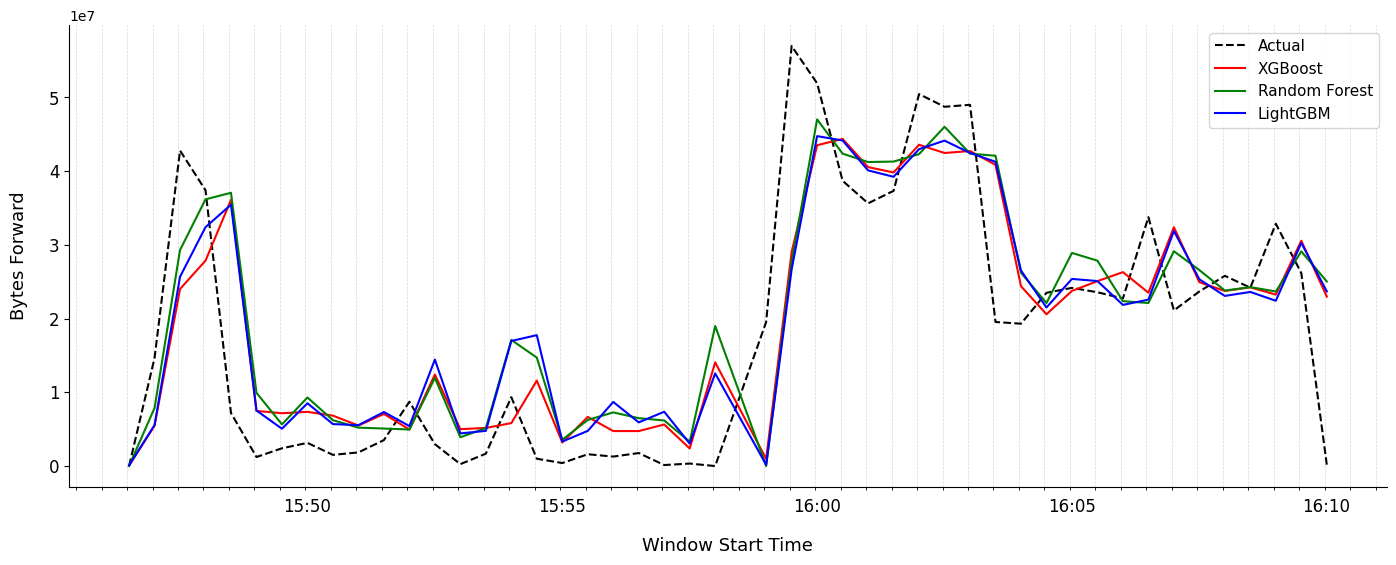
\includegraphics[width=0.9\textwidth]{resultados_30s.png}
    \caption{Comparison of model predictions with actual byte values for 30s time window}
    \label{fig:predictions_30s}
\end{figure}

\vspace{-10pt}

\begin{figure}[H]
    \centering
    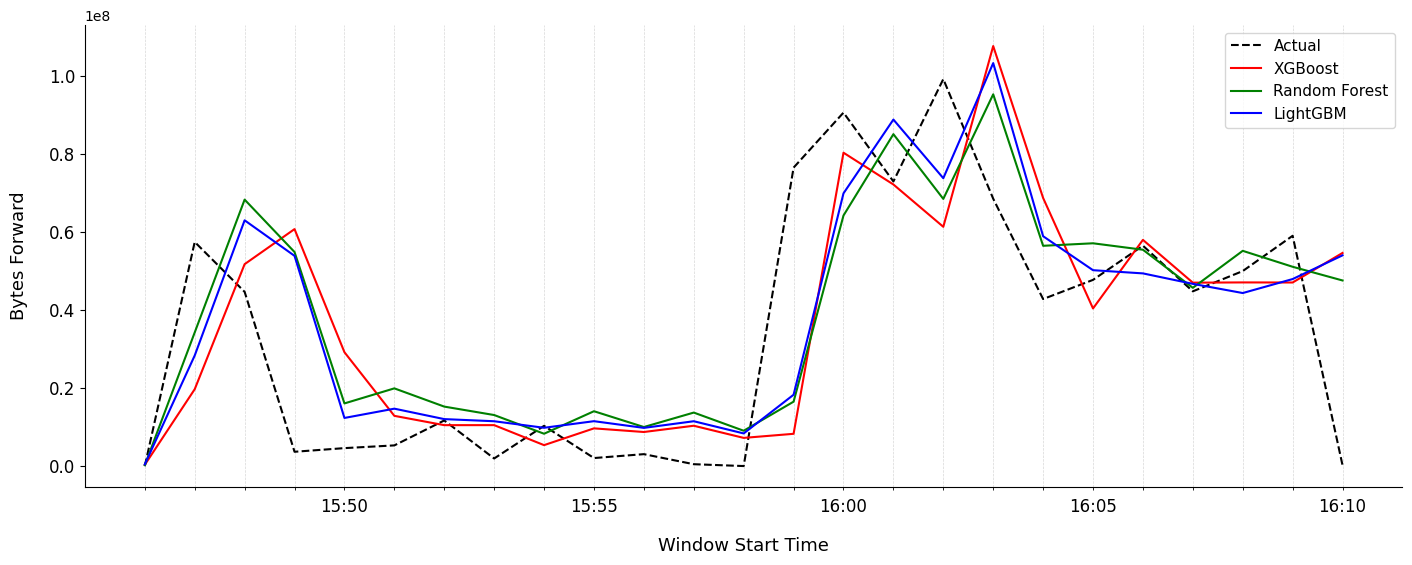
\includegraphics[width=0.9\textwidth]{resultados_1min.png}
    \caption{Comparison of model predictions with actual byte values for 1m time window}
    \label{fig:predictions_1m}
\end{figure}

\FloatBarrier

In terms of model comparison, all three models demonstrated similar predictive behavior, with LightGBM achieving the highest R² score for the 30-second window, while Random Forest performed best in the 1-minute setting. The relatively small variations in the R² values suggest that no single model outperformed the others by a substantial margin. However, the difference in performance between the two granularities suggests that finer time windows allow for a more accurate tracking of network traffic fluctuations, likely because the models have access to more frequent updates in the data.
%
%
\section{Conclusion}
The results showed that all models were able to capture the overall trends of network traffic but with a consistent lag of one time step in their predictions.
The comparison between granularities revealed that using a finer time window (30 seconds) resulted in higher predictive accuracy, as evidenced by the higher $R^2$ scores across all models. This suggests that shorter time intervals provide models with more detailed and responsive data, allowing them to better approximate real-time traffic fluctuations.


Although the models produced reasonable approximations of network traffic behavior, the observed lag in predictions remains a key limitation. This could indicate that the models rely too heavily on past observations without adequately adjusting to rapid shifts in traffic. Refining feature engineering or incorporating more temporally aware models could mitigate this issue. Deep learning approaches, such as Recurrent Neural Networks (RNNs) and Long Short-Term Memory (LSTM) networks, offer potential solutions by capturing long-term temporal patterns and dynamically adjusting to traffic changes.
%
%
%
%
%
%
%
% ---- Bibliography ----
%
% BibTeX users should specify bibliography style 'splncs04'.
% References will then be sorted and formatted in the correct style.
%
% \bibliographystyle{splncs04}
% \bibliography{mybibliography}
%

\section*{Acknowledgements}
This publication is part of the AI4SECIoT project ("Artificial Intelligence for Securing IoT Devices"), funded by the National Cybersecurity Institute (INCIBE), derived from a collaboration agreement signed between the National Institute of Cybersecurity (INCIBE) and the University of Burgos. This initiative is carried out within the framework of the Recovery, Transformation and Resilience Plan funds, financed by the European Union (Next Generation), the project of the Government of Spain that outlines the roadmap for the modernisation of the Spanish economy, the recovery of economic growth and job creation, for solid, inclusive and resilient economic reconstruction after the COVID‑19 crisis, and to respond to the challenges of the next decade.
\begin{thebibliography}{8}

\bibitem{ref_dataset1}
Neto, E.C.P., Dadkhah, S., Ferreira, R., Zohourian, A., Lu, R., Ghorbani, A.A.: CICIoT2023: A Real-Time Dataset and Benchmark for Large-Scale Attacks in IoT Environment. Sensors \textbf{23}(13), 5941 (2023). \doi{10.3390/s23135941}

\bibitem{ref_article1}
Leevy, J.L., Hancock, J., Zuech, R., et al., Detecting cybersecurity attacks across different network features and learners. J Big Data \textbf{8}, 38 (2021). \doi{10.1186/s40537-021-00426-w}

\bibitem{ref_article2}
Ahmed, M.A.O., AbdelSatar, Y., Alotaibi, R., Reyad, O.: Enhancing Internet of Things security using performance gradient boosting for network intrusion detection systems. Alexandria Engineering Journal \textbf{116}, 472--482 (2025). \doi{10.1016/j.aej.2024.12.106}

\bibitem{ref_article3}
Choudhury, A., Mondal, A. \& Sarkar, S.: Searches for the BSM scenarios at the LHC using decision tree-based machine learning algorithms: a comparative study and review of random forest, AdaBoost, XGBoost and LightGBM frameworks. Eur. Phys. J. Spec. Top. \textbf{233}, 2425–2463 (2024). \doi{10.1140/epjs/s11734-024-01308-x}

\end{thebibliography}

\end{document}
